\section{Gruppen}

\begin{definition}
    Sei $\mathfrak{G} = (G, \cdot, e, {}^{-1})$ eine Gruppe.
    \begin{itemize}
        \item Wir nennen $|G|$ die \emph{Ordnung} der Gruppe.\index{Gruppe!Ordnung}
        \item Sei $g \in G$, so erzeugt dieses Element eine Untergruppe
        $$ \langle \{ g \} \rangle = \{ g^n \mid n \in \mathbb{Z} \}. $$
        Wir nennen $|\langle\{g\}\rangle|$ die \emph{Ordnung} von $g$ und schreiben auch $\ord(g)$. Ist $\ord(g)$ endlich, so heißt $g$ \emph{Torsionselement}.\index{Gruppe!Torsionselement}
        \item $\mathfrak{G}$ heißt \emph{zyklisch}, falls es ein $g \in G$ mit $G = \langle\{g\}\rangle$ gibt.\index{Gruppe!zyklisch}
    \end{itemize}
\end{definition}

\begin{remark}
    Im Folgenden werden wir Gruppen durch ihre Trägermengen identifizieren. Für die Gruppe $\mathfrak{G, \cdot, e, {}^{-1}}$ wird oft nur $G$ geschrieben.
\end{remark}

\begin{example} {\ }
    \begin{enumerate}
        \item Betrachte $\mathbb{Z} \times \mathbb{Z}_m$, so ist $\ord(1,0) = \infty$ und $\ord(0,1) = m$.
        \item Betrachte $\mathbb{Z}_6$, so ist $\ord(1) = 6$, $\ord(2) = 3$ und $\ord(3) = 2$.
    \end{enumerate}
\end{example}

\begin{example} {\ }
    \begin{enumerate}
        \item Die Gruppen $(\mathbb{Z}, +, 0, -) = \langle\{1\}\rangle, (\mathbb{Z}_m, +, 0, -) = \langle\{1\}\rangle$ sind zyklisch.
        \item Die Gruppe $(\Gl_2(\mathbb{Q}), \cdot, E_2, {}^{-1})$ ist \emph{nicht} zyklisch, da -- wie wir noch sehen werden -- zyklische Gruppen abelsch sind.
    \end{enumerate}
\end{example}

\notedate{30.03.2023}

\begin{definition}
    Seien $G$ eine Gruppe, $U \le G$ eine Untergruppe und $g \in G$. Wir definieren 
    \begin{itemize}[topsep=0cm, label={--}]
        \item die \emph{Linksnebenklasse von $g$ nach $U$}\index{Linksnebenklasse} $gU := \{gu \mid u \in U\}$ und
        \item die \emph{Rechtsnebenklasse von $g$ nach $U$}\index{Rechtsnebenklasse} $Ug := \{ug \mid u \in U\}$.
    \end{itemize}
\end{definition}

\begin{lemma}\label{lemma:euqivrel_linksnebenklassen}
    Seien $G$ eine Gruppe, $U \le G$ eine Untergruppe und $g, g', x, y \in G$. Dann gilt:
    \begin{enumerate}
        \item Die Menge $\{gU \mid g \in G\}$ aller Linksnebenklassen von $g$ nach $U$ bildet eine Partition von $G$.
        \item Es gilt $gU = g'U$ genau dann, wenn $g^{-1}g' \in U$.
        \item Die Partition induziert eine Äquivalenzrelation $\sim$ auf $G$, wobei $x \sim y \Leftrightarrow \exists \tilde{g} \in G: x,y \in \tilde{g}U$.
        \item Es gilt für diese Äquivalenzrelation $x \sim y \Leftrightarrow x^{-1}y \in U$.\label{item:lemma:euqivrel_linksnebenklassen_4}
        \item Es ist $U = [e]_{\sim}$.
    \end{enumerate}
    
\end{lemma}
\begin{proof}{\ }
    \begin{enumerate}
        \item Es gilt $G = \bigcup_{g \in G} gU$, denn für $h \in G$ ist $h \in hU$, weil $e \in U$ und $h = h \cdot e$ ist. 
        
        Es bleibt noch zu zeigen, dass die Nebenklassen disjunkt sind. Dafür zeigen wir, dass nicht disjunkte Linksnebenklassen gleich sind. Seien also $g, g' \in G$ beliebig mit $gU \cap g'U \not= \emptyset$. Es existieren dann $u, u' \in U$, sodass $g u = g' u'$. Sei $a = g  u_a \in gU$ beliebig. Es ist dann $$ a = g u_a = g u u^{-1} u_a = g' \underbrace{u' u^{-1} u_a}_{\in U} \in g'U, $$
        also $gU \subseteq g'U$. Analog erhält man die andere Mengeninklusion, womit $gU = g'U$ gilt.
        \item Es ist 
        $$gU = g'U \;\Leftrightarrow\; \exists u, u' \in U: gu = g'u' \;\Leftrightarrow\; \exists u, u' \in U: u\left(u'\right)^{-1} = g^{-1}g' \;\Leftrightarrow\; g^{-1}g' \in U.$$
        \item Klarerweise wird durch eine Partition eine Äquivalenzrelation induziert. $\exists \tilde{g} \in G: x,y \in \tilde{g}U$ ist äquivalent dazu, dass $xU = yU$, was wiederum äquivalent dazu ist, dass $x, y$ die gleiche Äquivalenzklasse haben.
        \item \begin{itemize}[leftmargin=1cm]
            \item[``$\Rightarrow$'':] Es gibt $u, u' \in U$, sodass $x = g u$ und $y = g u'$. Es ist also $x^{-1} y = u^{-1} g^{-1} \cdot g  u' = u^{-1} u' \in U$.
            \item[``$\Leftarrow$'':] Es gilt $x^{-1}\cdot y = u$, also $y = x\cdot u$.  Es ist nun $x \in xU$ und auch  $y \in xU$, also $x \sim y$. 
        \end{itemize}
        \item Es ist $a \in [x]_\sim \;\Leftrightarrow\; e \sim x \;\Leftrightarrow\; e^{-1} a = a \in U $.
    \end{enumerate}
\end{proof}

\begin{remark}
    \cref{lemma:euqivrel_linksnebenklassen} gilt analog für Rechtsnebenklassen. Im Allgemeinen erhält man dabei allerdings eine andere Äquivalenzrelation.
\end{remark}

\begin{lemma}
    Seien $G$ eine Gruppe, $U \le G$ eine Untergruppe und $g \in G$. Es gilt $$\vert gU \vert = \vert U \vert = \vert Ug \vert.$$
\end{lemma}
\begin{proof}
    Definieren wir die Funktion $\varphi: U \to gU, u \mapsto g\cdot u$ und zeigen, dass sie bijektiv ist. Die Surjektivität ist klar, da $gU$ genau als das Bild von $\varphi$ definiert ist. Die Injektivtät erhalten wir wegen $gu = gu' \Rightarrow u = u'$. Damit ist $\vert U \vert = \vert gU \vert$. Die zweite Gleichheit wird analog gezeigt.
\end{proof}

\begin{remark}\label{rem:nebenklassenzerlegung_endlich}
    Ist $G$ eine endliche Gruppe, dann gilt $\vert G \vert = \vert \{gU \mid g \in G\} \vert \cdot \vert U \vert$, da alle Links-/Rechtsnebenklassen gleich mächtig sind. Durch umformen zu $\vert \{gU \mid g \in G\} \vert = \frac{\vert G \vert}{\vert U \vert}$ erhalten wir, dass es gleich viele Linksnebenklassen wie Rechtsnebenklassen gibt.

    \begin{figure}[H]
        \centering
        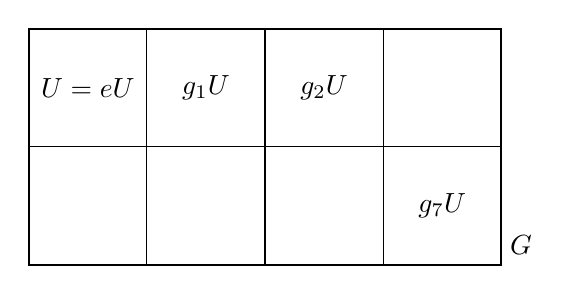
\begin{tikzpicture}
            \draw[thick] (0,0) rectangle (6, 3);
            \draw (0,1.5) -- (6,1.5) (1.5,0) -- (1.5,3) (3,0) -- (3,3) (4.5, 0) -- (4.5, 3);
            \node at (6.25, 0.25) {$G$};  
            \node at (0.75, 2.25) {$U = eU$};
            \node at (2.25, 2.25) {$g_1U$};
            \node at (3.75, 2.25) {$g_2U$};
            \node at (5.25, 0.75) {$g_7U$};
        \end{tikzpicture}
        \caption{Nebenklassenzerlegung einer endlichen Gruppe}
    \end{figure}
\end{remark}

\begin{remark}
    Es gilt auch für Gruppen mit unendlicher Trägermenge, dass es gleich viele Linksnebenklassen wie Rechtsnebenklassen gibt. Es kann dafür die Funktion $\varphi: gU \mapsto Ug^{-1}$ definiert werden und gezeigt werden, dass diese wohldefiniert und bijektiv ist.
\end{remark}

\begin{theorem}[Lagrange]\index{Satz!von Lagrange}
    Sei $G$ eine endliche Gruppe, $U \le G$ eine Untergruppe und $g \in G$. Dann gilt
    \begin{itemize}[topsep=0cm, label={--}]
        \item $\vert U \vert$ teilt $\vert G \vert$ und
        \item $\ord(g)$ teilt $\vert G \vert $.
    \end{itemize}
\end{theorem}
\begin{proof}
    Die erste Behauptung folgt aus \cref{rem:nebenklassenzerlegung_endlich}, für die zweite wählen wir $U := \langle g \rangle$.
\end{proof}

\begin{example}
    Betrachten wir $(\mathbb{Z}_6, +, 0, -)$ mit Ordnung 6. Es sind dann $\ord(0) = 1, \ord(1) = \ord(5) = 6, \ord(2) = \ord(4) = 3, \ord(3) = 2$, welche alle Teiler von 6 sind.

    Sei $G$ eine Gruppe mit $\vert G \vert = p \in \mathbb{P}$. Für $g \in G\setminus\{e\}$ gilt nun $\ord(g) = p \Rightarrow \langle g \rangle = G$, womit $G$ zyklisch ist. Gruppen mit Primzahlordnung sind also zyklisch.
\end{example}

\begin{definition}
    Sei $G$ eine Gruppe und $U \le G$ eine Untergruppe. Der \emph{Index von $U$ in $G$}\index{Index} ist definiert als $[G:U] := \vert \{gU \mid g \in G\}\vert = \vert \{Ug \mid g \in G\}\vert$. 
\end{definition}

\begin{remark}
    Ist $G$ endlich, dann haben wir in \cref{rem:nebenklassenzerlegung_endlich} $[G:U] = \frac{\vert G \vert}{\vert U \vert}$ gezeigt.
\end{remark}

\begin{theorem}[Indexsatz]\index{Indexsatz}
    Sei $G$ eine Gruppe und seien $U \le V \le G$ Untergruppen, dann ist $$[G:V] = [G:U] \cdot [U:V].$$ 
\end{theorem}
\begin{proof}
    Wurde in der Übung bewiesen.
\end{proof}

Im Allgemeinen ist die durch Links-/Rechtsnebengruppen induzierte Äquivalenzrelation keine Kongruenzrelation. Der folgende \cref{theorem:normalteiler_equiv} liefert Bedingungen, wann dies erfüllt ist.

\begin{definition}
    Sei $G$ eine Gruppe, dann heißt eine Teilmenge $N \subseteq G$ \emph{Normalteiler}\index{Normalteiler}, wenn eine der Bedingungen aus \cref{theorem:normalteiler_equiv} erfüllt ist. Man schreibt $N\vartriangleleft G$.
\end{definition}

\begin{theorem}\label{theorem:normalteiler_equiv}
    Sei $G$ eine Gruppe, $N \subseteq G$, dann sind äquivalent:
    \begin{enumerate}[label=(\enumArabicDual*)]
        \item\label{item:theorem:normalteiler_equiv_1} Es gibt genau eine Kongruenzrelation $\sim$ auf $G$ mit $N = [e]_\sim$, nämlich $x \sim y: \Leftrightarrow x^{-1}y \in N$.
        \item\label{item:theorem:normalteiler_equiv_1'} Es gibt eine Kongruenzrelation $\sim$ auf G mit $N = [e]_\sim$.
        \item\label{item:theorem:normalteiler_equiv_2} Es gibt eine Gruppe $H$ und einen surjektiven Homomorphismus $\varphi: G \to H$ mit $N = \varphi^{-1}(\{e_H\})$.
        \item\label{item:theorem:normalteiler_equiv_2'} Es gibt eine Gruppe $H$ und einen Homomorphismus $\varphi: G \to H$ mit $N = \varphi^{-1}(\{e_H\})$.
        \item\label{item:theorem:normalteiler_equiv_3} Es ist $N \le G$ mit $\forall x \in G: xNx^{-1} = N$.
        \item\label{item:theorem:normalteiler_equiv_3'} Es ist $N \le G$ mit $\forall x \in G: xNx^{-1} \subseteq N$.
        \item\label{item:theorem:normalteiler_equiv_4} Es ist $N \le G$ mit $\forall x \in G: xN = Nx$.
        \item\label{item:theorem:normalteiler_equiv_4'} Es ist $N \le G$ mit $\forall x \in G: xN \subseteq Nx$.
    \end{enumerate}
\end{theorem}


\begin{proof}{\ }
    \begin{itemize}[topsep=0cm, leftmargin=2.2cm]
        \item[\ref*{item:theorem:normalteiler_equiv_1} $\Rightarrow$ \ref*{item:theorem:normalteiler_equiv_1'}:] 
        Trivial.
        
        \item[\ref*{item:theorem:normalteiler_equiv_1'} $\Rightarrow$ \ref*{item:theorem:normalteiler_equiv_2}:] 
        Wählen wir $H = G/_\sim$ und sei $\varphi: G \to H, g \mapsto [g]_\sim$ die kanonische Einbettung. Es ist dann klarerweise $\varphi$ surjektiv und $\varphi^{-1}(\{e_H\}) = [e]_\sim = N$.
        
        \item[\ref*{item:theorem:normalteiler_equiv_2} $\Rightarrow$ \ref*{item:theorem:normalteiler_equiv_2'}:] 
        Trivial.
        
        \item[\ref*{item:theorem:normalteiler_equiv_2'} $\Rightarrow$ \ref*{item:theorem:normalteiler_equiv_3'}:] 
        Zeigen wir zuerst, dass $N$ eine Untergruppe ist. Seien dazu $n, n' \in N = \varphi^{-1}(\{e_H\})$. Dann ist $\varphi(n n') = \varphi(n) \varphi(n') = e_H e_H = e_H$, womit $n n' \in \varphi^{-1}(\{e_H\}) = N$ ist und damit $N \le G$.

        Zeigen wir nun noch für $x \in G, n \in N$, dass $y = xnx^{-1} \in N$ ist. Wir erhalten $$\varphi(y) = \varphi(x) \underbrace{\varphi(n)}_{= e_H} \varphi(x^{-1}) = \varphi(x)\varphi(x)^{-1} = e_H \;\Rightarrow\; y \in \varphi^{-1}(\{e_H\}) = N.$$

        \item[\ref*{item:theorem:normalteiler_equiv_3'} $\Rightarrow$ \ref*{item:theorem:normalteiler_equiv_3}:] 
        Wir wissen bereits, dass $\forall x \in G: xNx^{-1} \subseteq N$ gilt und wollen zeigen, dass für $y \in G$ die umgekehrte Inklusion gilt. Es ist $y^{-1} \in G$, womit $y^{-1}N(y^{-1})^{-1} = y^{-1}Ny \subseteq N$ ist. Wir erhalten damit nun 
        $$ N \overset{(*)}{=} y y^{-1} N y y^{-1} = y (y^{-1} N y) y^{-1} \subseteq y N y^{-1}, $$
        wobei $(*)$ einfach nachzurechnen ist.
        
        \item[\ref*{item:theorem:normalteiler_equiv_3} $\Rightarrow$ \ref*{item:theorem:normalteiler_equiv_4}:] 
        Zeigen wir für $x \in G$, dass $xN \subseteq Nx$ ist. Für ein $y \in xN$ gibt es ein $n \in N$, sodass $y = xn$. Wählen wir $n' = yx^{-1} = xnx^{-1} \in xNx^{-1} = N$, so ist $y = n'x$ und damit $y \in Nx$. Die andere Mengeninklusion zeigt man analog. 
        
        \item[\ref*{item:theorem:normalteiler_equiv_4} $\Rightarrow$ \ref*{item:theorem:normalteiler_equiv_4'}:] 
        Trivial.
        
        \item[\ref*{item:theorem:normalteiler_equiv_4'} $\Rightarrow$ \ref*{item:theorem:normalteiler_equiv_1}:]  
        Zeigen wir zuerst die Eindeutigkeit: Sei angenommen es gibt eine Kongruenzrelation $\sim$ auf $G$ mit $N = [e]_\sim$. Für $x, y\in G$ gilt dann 
        \begin{itemize}[label={--}]
            \item $x \sim y \;\Rightarrow\; x^{-1}x \sim x^{-1}y \; \Leftrightarrow\; e \sim x^{-1}y \;\Leftrightarrow\; x^{-1}y \in [e]_\sim = N$ und
            \item $x^{-1}y \in N = [e]_\sim \;\Leftrightarrow\; e \sim x^{-1}y \;\Leftrightarrow\; x = xe \sim x(x^{-1}y) = y$.
        \end{itemize}
        Es ist dann also $x \sim y \Leftrightarrow x^{-1}y \in N$. 
        
        Zeigen wir nun noch, dass dieses $\sim$ eine Kongruenzrelation auf $G$ ist. Nach \cref{lemma:euqivrel_linksnebenklassen} ist $\sim$ eine Äquivalenzrelation, bleibt also noch die Invarianz unter $G$ zu zeigen. 
        \begin{itemize}[label={--}]
            \item Zeigen wir für $x,x',y,y' \in G$ mit $x \sim y, x' \sim y'$, dass $xx'\sim yy'$. Es gilt 
            $$ xx'\sim yy' \;\Leftrightarrow\; x'^{-1}\underbrace{x^{-1}y}_{=: n \in N} y' = \underbrace{x'^{-1} n}_{\in x'^{-1}N \subseteq Nx'{-1}} y' \overset{(*)}{=} n'\underbrace{x'^{-1}y'}_{\in N} \in N, $$
            wobei wir bei $(*)$ verwenden, dass nach \ref*{item:theorem:normalteiler_equiv_4'} ein $n' \in N$ existiert, sodass $x'{-1} n = n' x'{-1}$.
            \item Zeigen wir für $x,y \in G$ mit $x \sim y$, dass $x^{-1} \sim y^{-1}$. Es gilt
            $$ x\sim y \;\Leftrightarrow\; x^{-1}x \sim x^{-1}y \;\Leftrightarrow\; e \sim x^{-1}y \;\Leftrightarrow\; ey^{-1} \sim x^{-1} y y^{-1} \;\Leftrightarrow\; y^{-1} \sim x^{-1}.$$ 
            \item Klarerweise ist $e \sim e$, also ist $\sim$ invariant unter der 0-stelligen Operation $e$.
        \end{itemize}
    \end{itemize}
\end{proof}

\begin{remark}
    \cref{theorem:normalteiler_equiv} beschreibt einige Eigenschaften von Normalteilern.
    \begin{itemize}[label={--}]
        \item \ref*{item:theorem:normalteiler_equiv_1}, \ref*{item:theorem:normalteiler_equiv_1'} liefern den bijektiven Zusammenhang von Normalteilern und Kongruenzrelation. Betrachtet man die Verbände von Normalteilern bzw. Kongruenzrelationen, so stellt diese Bijektion einen Verbandsisomorphismus dar.
        \item \ref*{item:theorem:normalteiler_equiv_2}, \ref*{item:theorem:normalteiler_equiv_2'} beschreiben die Darstellung des Normalteilers über den Kern eines Homomorphismus $\varphi: G \to H$. Es ist $\ker \varphi = \{g \in G \mid \varphi(g) = e_H\} = \varphi^{-1}(\{e_H\}) = N$.\footnote{Hier besteht eine Ähnlichkeit zum Kern von linearen Abbildungen der ein Unterraum ist.}
        \item \ref*{item:theorem:normalteiler_equiv_3}, \ref*{item:theorem:normalteiler_equiv_3'} liefern direkt, dass Normalteiler unter Abbildungen $\pi_x: G \to G, g \mapsto xgx^{-1}$ abgeschlossen sind. So eine Abbildung nennt man \emph{inneren Automorphismus}.
        \item \ref*{item:theorem:normalteiler_equiv_4}, \ref*{item:theorem:normalteiler_equiv_4'} besagen, dass die Links- und Rechtsnebenklassen genau dann gleich sind, wenn die Untergruppe ein Normalteiler ist.
    \end{itemize}
\end{remark}

\begin{corollary}
    In einer abelschen Gruppe $G$ ist $N \subseteq G$ genau dann ein Normalteiler, wenn $N$ eine Untergruppe von $G$ ist.
\end{corollary}
\begin{proof}
    In einer abelschen Gruppe ist immer $xN = Nx$. \cref{theorem:normalteiler_equiv} \ref*{item:theorem:normalteiler_equiv_4} liefert dann damit die Behauptung.
\end{proof}